
%(BEGIN_QUESTION)
% Copyright 2013, Tony R. Kuphaldt, released under the Creative Commons Attribution License (v 1.0)
% This means you may do almost anything with this work of mine, so long as you give me proper credit

Suppose a Siemens S7-200 PLC is loaded with the following program utilizing a ``Count Up'' (CTU) instruction:

$$\includegraphics[width=15.5cm]{i02854x01.eps}$$

Assuming this counter's current value (CV) happens to be 7 at the point in time where we begin to monitor its operation, predict its current value at the following points in time given the input conditions shown by this pulse diagram:

$$\includegraphics[width=15.5cm]{i02854x02.eps}$$

Note that a ``high'' logic state represents a condition where that PLC input channel is electrically energized, while a ``low'' logic state represents a de-energized condition.

\vskip 10pt

CV at time ``A'' = \underbar{\hskip 50pt} 

\vskip 10pt

CV at time ``B'' = \underbar{\hskip 50pt} 

\vskip 10pt

CV at time ``C'' = \underbar{\hskip 50pt} 

\vskip 10pt

CV at time ``D'' = \underbar{\hskip 50pt} 

\vskip 10pt

CV at time ``E'' = \underbar{\hskip 50pt} 

\underbar{file i02854}
%(END_QUESTION)





%(BEGIN_ANSWER)

CV at time ``A'' = \underbar{\bf 7} 

\vskip 10pt

CV at time ``B'' = \underbar{\bf 8} 

\vskip 10pt

CV at time ``C'' = \underbar{\bf 1} 

\vskip 10pt

CV at time ``D'' = \underbar{\bf 4} 

\vskip 10pt

CV at time ``E'' = \underbar{\bf 0} 

%(END_ANSWER)





%(BEGIN_NOTES)

{\bf This question is intended for exams only and not worksheets!}.

%(END_NOTES)


